\documentclass{article}
\usepackage[utf8]{inputenc}
\usepackage{amsmath}
\usepackage{amssymb}
\usepackage{graphicx}
\usepackage{wrapfig}

\graphicspath{{Images/}}

\setlength{\oddsidemargin}{0in}
\setlength{\textwidth}{6.5in}
\setlength{\topmargin}{-.55in}
\setlength{\textheight}{9in}
\pagestyle{empty}


\title{Solid State Take Home Exam 2}
\author{Michael Nameika}
\date{November 2022}

\begin{document}

\maketitle

\section*{Problem 1}
The interaction energy between two atoms may be described by 
\[U(r) = \frac{A}{r^n} - \frac{B}{r^m}\]
Show that the molecule will break up when the atoms are pulled apart to a distance
\[r_b = r_0\left(\frac{n+1}{m+1}\right)^{1/(n-m)}\]
where $r_0$ is the equilibrium distance between the atoms. Discuss the criterion of braking used to get the above result.
\newline\newline
To begin, let us calculate the equilibrium distance. The equilibrium distance will be given when $dU/dr = 0$: 
\begin{align*}
    \frac{dU}{dr} &= -\frac{nA}{r_0^{n+1}} + \frac{mB}{r_0^{m+1}} = 0\\
    \frac{nA}{r_0^{n+1}} &= \frac{mB}{r_0^{m+1}} \\
    \frac{r_0^{m+1}}{r_0^{n+1}} &= \frac{mB}{nA} \\
    r_0^{m - n} &= \frac{mB}{nA} \\
    r_0 &= \left(\frac{mB}{nA}\right)^{1/(m-n)} \\
    &= \left(\frac{nA}{mB}\right)^{1/(n-m)} \\
\end{align*}
Now, I claim that the molecule will break apart when the atoms are pulled apart to a distance $r_b$ such that $d^2U/dr^2|r = r_b = 0$. Let us calculate $d^2U/dr^2$ and set it equal to zero:
\begin{align*}
    \frac{d^2U}{dr^2} &= \frac{n(n+1)}{r_b^{n+2}}A - \frac{m(m+1)}{r_b^{m+2}}B = 0 \\
    \frac{n(n+1)}{r_b^{n+2}}A &= \frac{m(m+1)}{r_b^{m+2}}B \\
    r_b^{m-n} &= \frac{m(m+1)B}{n(n+1)A} \\
    r_b &= \left(\frac{m(m+1)B}{n(n+1)A}\right)^{1/(m-n)} \\
    &= \left(\frac{n(n+1)A}{m(m+1)B}\right)^{1/(n-m)} \\
    &= \left(\frac{nA}{mB}\right)^{1/(n-m)}\left(\frac{n+1}{m+1}\right)^{1/(n-m)} \\
    &= r_0\left(\frac{n+1}{m+1}\right)^{1/(n-m)} \\
\end{align*}
So we have $r_b = r_0\left(\frac{n+1}{m+1}\right)^{1/(n-m)}$ which is what we wanted to show. 

This criterion of requiring the second derivative to be equal to zero is requiring that there is no work being done by the repulsive and Coulomb forces since work is related to the second spacial derivative of potential. 

\section*{Problem 2}
The mean energy of each vibrational mode is given as:
\[E = \hbar\omega\left[\frac{1}{2} + n(\omega, T)\right]\]
where $n(\omega, T)$ is the number of phonons with frequency $\omega$ at temperature $T$. In class, we showed that in the high-temperature limit, the energy of a single vibration is given as
\[E = \hbar\omega\left[\frac{1}{2} + n(\omega, T)\right] = k_BT\]
under the assumption that $\hbar\omega \ll k_BT$. Calculate the relative error in the internal energy in the high-temperature approximation when $\hbar\omega = k_BT$. Provide an answer with 4 significant figures!
\newline\newline
To begin, recall that relative error ($RE$) is given by
\[RE = \frac{|\text{Approximate Value} - \text{True Value}|}{\text{True Value}}\]
Here, our approximate value is $E = k_BT$ and our true value is $E = k_BT\left(\frac{1}{2} + n(\omega, T)\right)$. Recall that the time average for $n$ is given by $\langle n \rangle = \frac{1}{\exp{(\hbar\omega/k_BT)}-1}$. And for the high temperature limit $\hbar\omega = k_BT$, we have $\langle n \rangle = \frac{1}{e-1}$ Now, using these to calculate the relative error, we find
\begin{align*}
    RE &= \frac{k_BT(\frac{1}{2} + n(\omega, T)) - k_BT}{k_BT(\frac{1}{2} + n(\omega, T))} \\
    &= \frac{\frac{1}{e-1} - \frac{1}{2}}{\frac{1}{2} + \frac{1}{e - 1}} \\
    &\approx 7.577 \times 10^{-2} \\
\end{align*}
So the error is just below 8\%.



\section*{Problem 3}
\begin{wrapfigure}{R}{0.3\textwidth}
    \begin{center}
        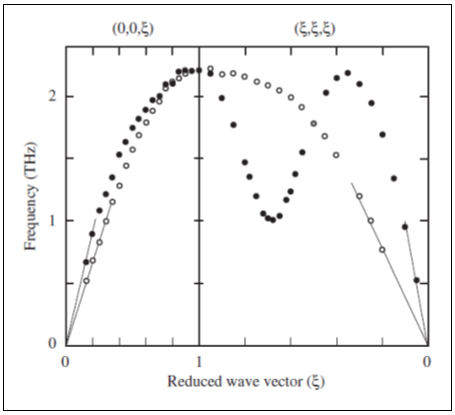
\includegraphics[width = 0.4\textwidth]{single frequency mode.PNG}
    \end{center}
\end{wrapfigure}
You may recall that in class I have shown you and discuss with you dispersion relation for bcc potassium. 
It is a figure to the right which you have seen already. 
Look at the more complete data set for potassium taken at 9 K on the next page. 
Based on these data, sketch the density of states for potassium in arbitrary units. For each local (global) maximum and minimum write a sentence or two on why it occurs!
It will be interesting to compare your conclusions (sketch) with the actual calculations where the authors have taken into account interactions with up to $5^{\text{th}}$ nearest neighbors and over 60 000 000 normal modes! Here is new data.
\newline\newline
\begin{center}
    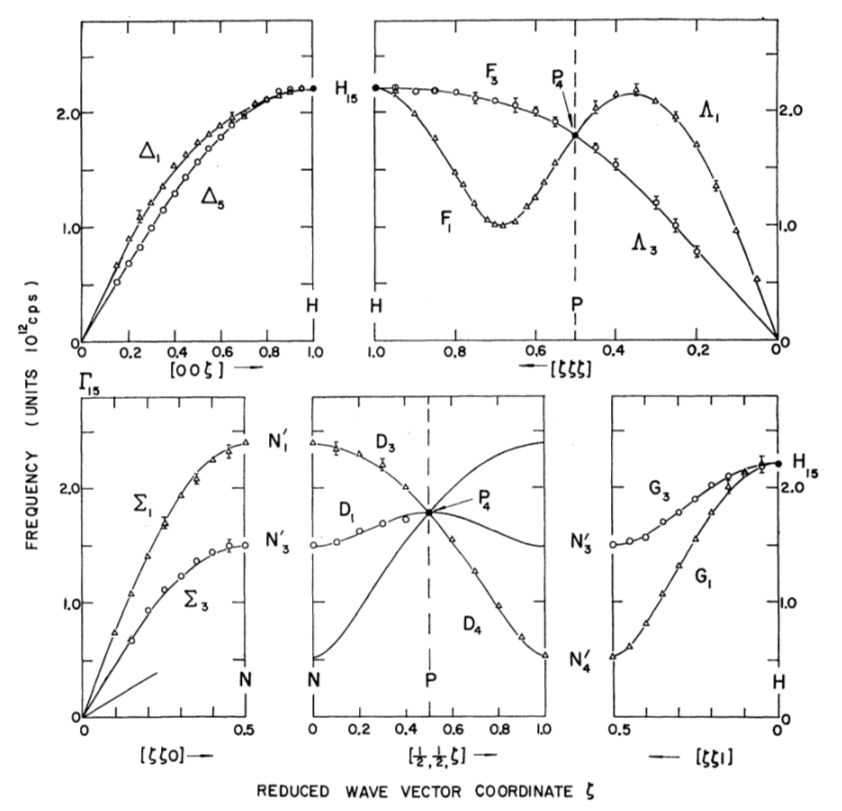
\includegraphics[scale = 0.6]{frequency modes.PNG}
\end{center}
To begin, recall that the density of states is related to the dispersion relation by the following formula:
\[\mathcal{D}(\omega)d\omega = \left(\frac{L}{2\pi}\right)^3\int_{\text{shell}}d^3K\]
That is, for each of the plots above for the given planes, we estimate the shape of the density of states for each plane by thinking about taking the one dimensional integral of the given plots above. 
That is, we can sketch a curve whose slope is given by the graphs of the dispersion relation.
See the attached sketches below.


The maxima and minima occur at the boundaries of the boundaries of the first Brillouin zone. 
More explicitly, we have that at the value of $k = 0$, the minimum value of the density of states occurs and at $k = \pi/L$. 
For $k = 0$, we have that there is no vibration in the lattice, so we should expect there to be no modes, so the density of states should be zero, which is exactly what we see. 
At the boundary, we see the highest frequency, from which we should expect the highest number of modes, which is exactly what we see.

\section*{Problem 4}
Using data from figures below determine the velocity of sound in Si at 20K and $0^{\circ}$C. $(R = 8.314 \text{J}/(\text{K mol})$. Si lattice constant is 0.5431 nm. Assume that phonon mean free path is a linear function of temperature. Its values at 77 and 250 K are 80 and 13 microns respectively. For Si $\Theta_{\text{D}} = 640$K.
\begin{center}
    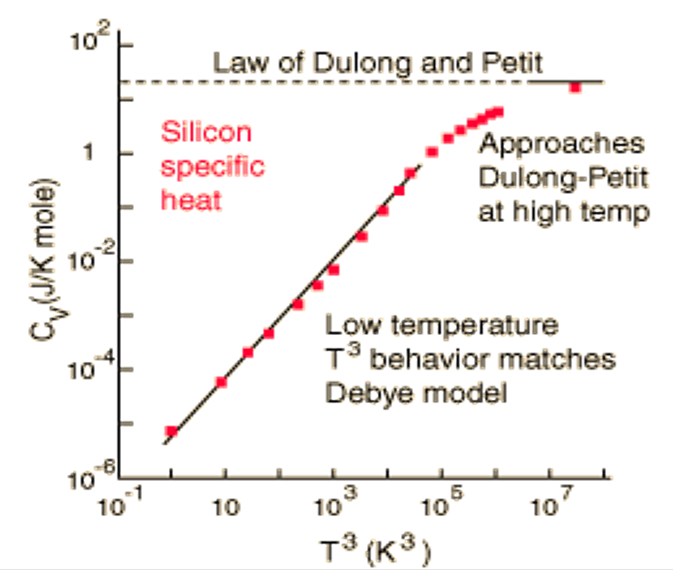
\includegraphics[scale = 0.6]{dulong.PNG}
    \newline
    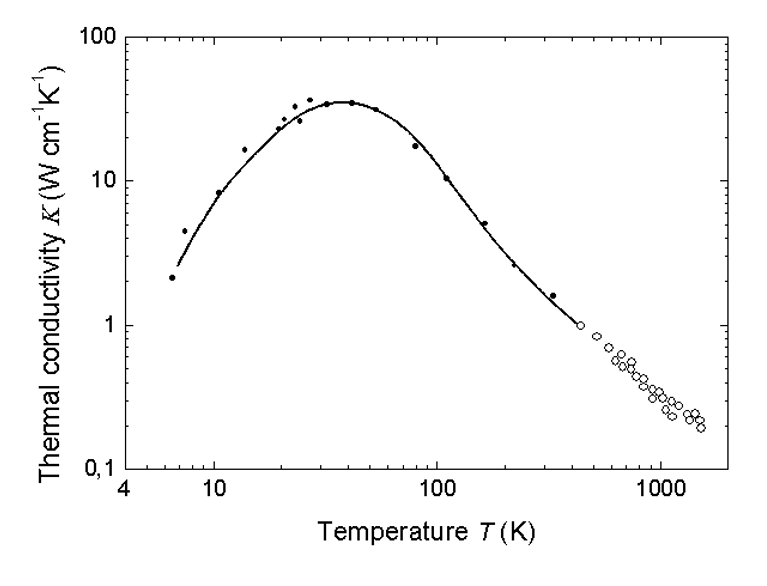
\includegraphics[scale = 0.6]{thermal conductivity.PNG}
\end{center}
Recall that the following formula that relates specific heat and speed of sound:
\[v^3 = \frac{3V\hbar^2}{2\pi^2C_Vk_BT^2}\int_0^{\omega_D}\frac{\omega^4e^{\hbar\omega/k_BT}}{(e^{\hbar\omega/k_BT} - 1)^2}d\omega\]
making the substitution $x = \omega\hbar/k_BT$, the above equation turns to
\[v^3 = \frac{3VNk_B^4T^3}{2\pi^2C_v\hbar^3}\int_0^{x_D}\frac{x^4e^x}{(e^x + 1)^2}dx\]
where $x_D = \Theta_D/T$ and $N$ in the numerator is Avogadro's number, to compensate for the fact that $[C_V] = \text{ J mol}^{-1}\text{K}^{-1}$. And for $T = 20 \text{ K}$, we have $x_D = 32$.
\newline
Further recall that $C_V$ may be estimated by $C_V \approx 234Nk_B(T/\theta)^3$. For $T = 20K$ and $\theta = 640$, we have $C_V \approx .0594 \text{ J/(mol K)}$.
\newline
Now, since our lattice parameter is $a = 0.5431 \text{ nm}$, we have $V = (0.5431 \times 10^{-9} \text{ m})^3 = 1.6019 \times 10^{-28} \text{ m}^3$. Additionally, we have $\hbar/(k_BT) = 3.38192\times 10^{-13} \text{ s}$. 
Plugging these values into the equation we have for velocity, we have
\begin{align*}
    v^3 &= \frac{3*(1.6019\times 10^{-28} \text{ m}^3)\hbar^2(6.02214\times 10^{23} \text{ mol})}{2\pi^2(0.0594 \text{J}/\text{(mol K)}k_B(20 \text{ K})^2)}\int_0^{32}\frac{x^4e^{x}}{(e^{x} - 1)^2}dx \\
    &\approx 1.5896\times 10^{12} \frac{\text{m}^3}{\text{s}^3} \\
    v &= 1.1671\times 10^4 \frac{\text{m}}{\text{s}} \\
\end{align*}
So the speed of sound in silicon at 20 K is approximately $1.1671 \times 10^4 $ m/s.
\newline

Now, for $T = 0^{\circ} \text{ C} = 273.15 \text{ K}$, we have 
\[\frac{\hbar}{k_BT} = 2.7964\times 10^{-14}\]
and estimate $C_V \approx R = 8.3145 \text{ J mol}^{-1}\text{ K}^{-1}$.
\newline
And so our equation for velocity becomes
\begin{align*}
    v^3 &= \frac{3*(1.6019\times 10^{-28} \text{ m}^3)\hbar^2(6.02214\times 10^{23} \text{ mol})}{2\pi^2(8.3145 \text{J}/\text{(mol K)}k_B(273.15 \text{ K})^2}\int_0^{\frac{640}{273.15}}\frac{x^4e^{x}}{(e^{x} - 1)^2}dx\\
    &\approx 3.6823\times 10^{12} \frac{\text{m}^3}{\text{s}^3} \\
    v &= 1.5442\times 10^4 \frac{\text{m}}{\text{s}} \\
\end{align*}
So the velocity of sound in silicon at room temperature is approximately $1.5442\times 10^4$ m/s.
\end{document}
